\documentclass[11pt]{article}

\usepackage[margin=1in]{geometry}
\usepackage{parskip}
\usepackage{amsmath}
\usepackage[style=ieee]{biblatex}
\usepackage{graphicx}
\usepackage{wrapfig}
\usepackage{float}
\usepackage{caption}

\graphicspath{{./images/}}

\addbibresource{ia.bib}

\begin{document}

\title{Applying State Space Control and LQR to the Pole Balancing Problem}
\author{Brendon Matusch}
\date{November 2018}
\maketitle

\section{Introduction}

\subsection{The Pole Balancing Problem} \label{problem}

One of the most famous problems in control theory is the \textit{pole balancing problem}, also known as \textit{cart pole}. The basic idea of the problem is as follows:

\begin{itemize}
    \item A movable cart with mass $M$ sits on a two-dimensional, straight track, at horizontal position $x _c$.
    \item A pole with length $l$ is anchored to the cart with a hinge at angle $\theta$ (which can change).
    \item A weight with mass $m$ is attached to the end of the pole.
    \item A motor can accelerate the cart to the left or right with force $F$.
    \item Gravity, which applies downward force $g$, is present.
    \item The goal is to prevent the pole from falling over (to prevent $\theta$ from becoming too large), while also keeping the cart near the center of the track (keeping $x _c$ small).
\end{itemize}

\begin{figure}[ht]
    \centering
    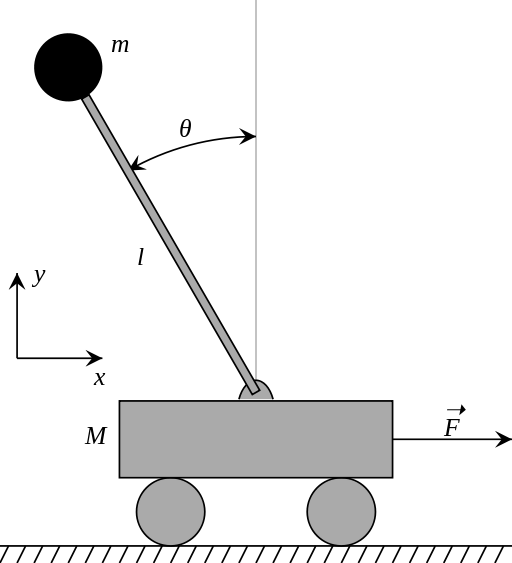
\includegraphics[width=0.5\textwidth]{cartpole}
    \caption{\label{cartpole} A diagram of the pole balancing problem.}
\end{figure}

I hoped to solve the pole balancing problem in an efficient way, because a solution to this problem has many applications in a variety of fields. For instance, control of many kinds of robots (such as two-wheeled vehicles and walking humanoid robots) is closely related to the pole balancing problem. All the concepts I have learned throughout developing a solution to this problem are applicable to challenges in robotics, some of which I hope to approach in the future.

The pole balancing problem, as visualized in Figure \ref{cartpole}, is quite clearly not trivial. If the pole starts to fall to the right, one must accelerate the cart to the right to prevent it from falling over. However, that also results in the cart moving away from the center. Thus, to successfully optimize both the angle and the position, one must gradually adjust the angle by applying small forces while the cart moves.

\subsection{Control Algorithms}

I started by researching the most common control algorithms for this kind of control challenge. The most frequently used method I encountered, both in my past experience and in my research, was the PID (proportional, integral, and derivative) closed control loop. However, I discovered that PID loops are only able to optimize one variable at a time (for instance, the angle of the pole, or the position of the cart). Optimizing multiple variables (as is required here) necessitates nesting of PID loops, which frequently have to be optimized either manually or via machine learning.

An alternative control method I encountered in my research, which can optimize multiple variables with one or more inputs, is state space control. Rather than dealing with only a single variable, state space controllers can optimize an entire vector of states in a single linear function, making for a simpler and more elegant solution.

Additionally, and more importantly, I discovered that state space controllers can be automatically optimized using a method known as Linear-Quadratic Regulator (LQR). While I found it surprising that LQR is such an automatic method, further research confirmed my findings. All that is required is a linear model of the environment expressed in matrices.

For this project, I have created a mathematical model of the pole balancing problem and developed a state space controller to effectively optimize it. While this was a challenging endeavor and I had to learn a lot of new mathematics, I am very happy with the result.

\section{Environment}

\subsection{Equations of Motion} \label{equations}

In order to develop a solution to the pole-balancing problem, I first had to model it. Creating a physical cart pole setup would have taken a long time, so I used a simulated model instead. In order to develop this, I used the differential equations of motion for the pole balancing problem, which I found at \cite{polebalancing}:

\begin{equation}
    \ddot \theta = \frac{\displaystyle g \sin \theta + \cos \theta \left( \frac{\displaystyle -F - m l \dot \theta ^2 \sin \theta}{\displaystyle M + m} \right)}{\displaystyle l \left( \frac{\displaystyle 4}{\displaystyle 3} - \frac{\displaystyle m \cos ^2 \theta}{\displaystyle M + m} \right)}
\end{equation}

\begin{equation}
    \ddot x _c = \frac{\displaystyle F + m l \left( \dot \theta ^2 \sin \theta - \ddot \theta \cos \theta \right)}{\displaystyle M + m}
\end{equation}

Note the use of dot-derivative notation, where $\displaystyle \dot \theta = \frac{\displaystyle d \theta}{\displaystyle d t}$ (the first derivative of $\theta$) and $\displaystyle \ddot \theta = \frac{\displaystyle d ^2 \theta}{\displaystyle d t ^2}$ (the second derivative of $\theta$, and the first derivative of $\dot \theta$), and respectively for $x _c$.

That is, $\dot \theta$ is the rate at which $\theta$ is changing in radians per second, and $\ddot \theta$ is the rate at which $\dot \theta$ is changing in radians per second squared.

\subsection{Implementation}

Of course, it would not be possible to run such a simulation with many variables on a calculator, so I wrote a program instead. I implemented these equations of motion in Python 3 using NumPy \cite{numpy}, which is a commonly used library for basic linear algebra operations like matrix multiplications. I have used NumPy numerous times in the past for tasks such as machine learning, so I was quite familiar with it.

The following values were used for the various constants of the system:

\begin{itemize}
    \item $M = 1$
    \item $m = 0.1$
    \item $l = 0.5$
    \item $g = 9.81$
\end{itemize}

The differential equations of motion refer to a continuous environment, where acceleration, position, and velocity values change every instant. Since this is impossible to compute in reality, I implemented the system with a time step of 0.001 (meaning that all variables of motion are updated every 0.001 time units).

While all equations work with arbitrary units, in this paper all variables and quantities are assumed to be in SI units (seconds, meters, kilograms, and radians).

\subsection{Visualization}

\subsubsection{Animated Visualization Tool}

To make the model more easy to visualize and understand, I developed an animated visualization tool using PyQt5 (Figure \ref{simulation}). It displays the cart and pole as rectangles on top of the linear track.

\begin{figure}[ht]
    \centering
    
\includegraphics[width=\textwidth]{simulation}
    \caption{\label{simulation} A screenshot of the animated visualization tool.}
\end{figure}

\subsubsection{Motion Plots}

For more precise static visualization of potential problems with control algorithms, I used Matplotlib \cite{matplotlib} to create plots over time of $x _c$, $\theta$, and $F$. These plots are seen in Figures \ref{position}, \ref{angle}, and \ref{force} at the end of this paper. Following are some specific issues this tool can help to shed light on:

\begin{itemize}
    \item Overshooting: when, rather than gradually settling to a stable equilibrium, the controller accelerates the cart and does not slow down enough to slow down and stop at 0. Mathematically, a controller that does not overshoot has a limit of 0 and is strictly increasing (if the starting $x _c$ is below 0) or strictly decreasing (if the starting $x _c$ is above 0).
    \item Excessive acceleration: rapid jumps or spikes in any of the variables in question may indicate strange and unwanted behavior, which may be attributable to poor parameter choices or modeling errors.
\end{itemize}

\section{State Space}

\subsection{Concepts}

I learned about state space control from a book \cite{veness} written by Tyler Veness, a FIRST Robotics Competition mentor. I used the knowledge I gained in this book to develop a state space control algorithm that works for the pole balancing problem. The basic concepts of state space control are as follows:

\begin{enumerate}
    \item States of the environment to be controlled are expressed in a constantly changing state vector $\vec{x}$ (not to be confused with the horizontal position $x _c$).
    \item Inputs to the system are provided as an input vector $\vec{u}$.
    \item The derivative of the state vector, $\dot{\vec{x}}$, is defined by the following equation:
        \begin{equation} \label{state_derivative}
            \dot{\vec{x}} = A x + B u
        \end{equation}
        The two matrices used in this equation represent a linear model of the environment as follows:
        \begin{itemize}
            \item The system matrix $A$ with size (states $\times$ states) defines how the states automatically change over time (in dynamics such as gravity).
            \item The input matrix $B$ with size (states $\times$ inputs) defines how the inputs provided by a control algorithm influence the changing states of the environment.
        \end{itemize}
        Figure \ref{state_space} illustrates the flow of data as described by this equation.
        \begin{figure}[ht]
            \centering
            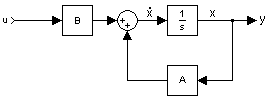
\includegraphics[width=0.5\textwidth]{state_space}
            \caption{\label{state_space} A flow chart describing changes in a state space environment.}
        \end{figure}
    \item The basic control law of state space is as follows:
        \begin{equation} \label{control_law}
            \vec{u} = K(\vec{r} - \vec{x})
        \end{equation}
        The \textit{reference} vector, which contains the values we hope to drive the states to, is written as $\vec{r}$. If the goal is to minimize the states, it will be a vector of zeroes. $K$ is the \textit{controller gain} matrix, of size (inputs $\times$ states). It is multiplied by the state error $\vec{r} - \vec{x}$ to produce a (hopefully) optimal input to drive the states to the reference.
\end{enumerate}

\subsection{Implementation}

\subsubsection{States and Inputs}

The first step in developing a state space control algorithm was to express the environment in state space notation. This means choosing a vector of states and a vector of inputs that fully define the cart pole system.

The physical dynamics can be fully described with only four parameters: $\theta$ (which determines the action of gravity), $\dot \theta$ (which defines the momentum of the pole), $x _c$ (the distance along the track), and $\dot x _c$ (the momentum of the cart). These are the only non-constant parameters used in the differential equations of motion in Section \ref{equations}. Thus:

\begin{equation}
    \displaystyle \vec{x} = \begin{bmatrix}
        \theta \\
        \dot \theta \\
        x _c \\
        \dot x _c
    \end{bmatrix}
\end{equation}

While there are four states required to describe the environment, there is only one parameter the controller has access to, and that is the force applied to the cart. Thus:

\begin{equation}
    \vec{u} = \begin{bmatrix}
        \displaystyle F
    \end{bmatrix}
\end{equation}

\subsubsection{Linearization}

Since the full behavior of the environment is described in two constant matrices ($A$ and $B$), and matrix multiplication is a linear operation, the environment must actually be linear to use standard state space control.

Thankfully, I realized that $\theta$ will always be small (otherwise, the cart would either fall over, or have to constantly accelerate very rapidly). If $\theta$ is small, the nonlinear trigonometric ratios can be approximated as linear functions with minimal error. Specifically, when $\theta$ is small, $\sin \theta \approx \theta$ and $\cos \theta \approx 1$. I took advantage of these facts to linearize the pole balancing problem, as follows:

\begin{itemize}
    \item The torque applied by gravity on the arm is equal to $\displaystyle \frac{\displaystyle g \sin \theta}{\displaystyle l}$, which can be linearly approximated as $\displaystyle \frac{\displaystyle g \theta}{\displaystyle l}$ for values of $\theta$ near 0.
    \item The torque applied by horizontal acceleration of the cart on the arm (assuming the arm is of negligible mass) is equal to $\displaystyle - \frac{\displaystyle F \cos \theta}{\displaystyle l}$, which can be linearly approximated as $\displaystyle - \frac{\displaystyle F}{\displaystyle l}$ for values of $\theta$ near 0.
    \item The acceleration applied to the cart by a force is simply equal to $\displaystyle \frac{\displaystyle F}{\displaystyle M + m}$ (once again, under the assumption that the pole mass is negligible).
    \item The only dynamics other than gravity and force that must be modeled are the influences of the velocity states $\dot \theta$ on $\theta$ and $\dot x _c$ on $x _c$. These are obviously linear.
\end{itemize}

\begin{figure}[ht]
    \centering
    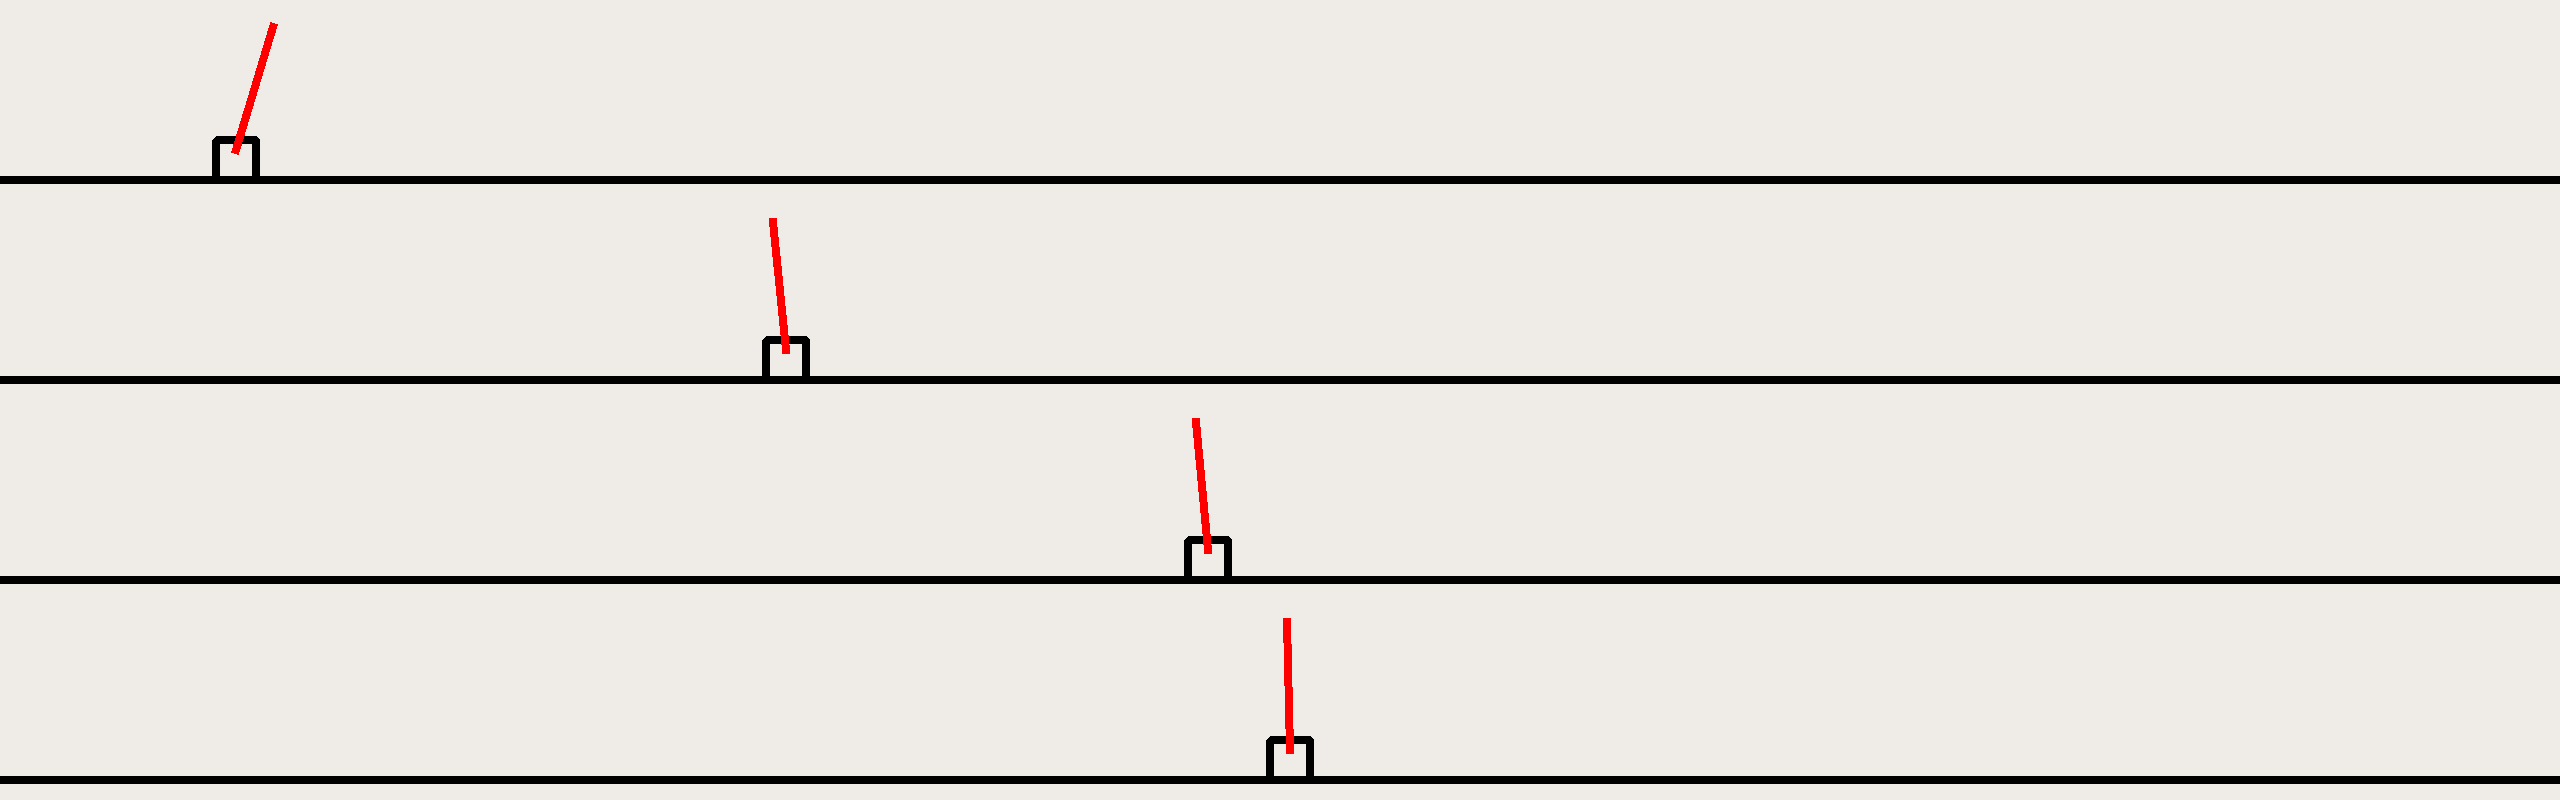
\includegraphics[width=\textwidth]{animation}
    \caption{\label{animation} An example run of the simulation, showing that even during periods of fast movement, $\theta$ remains fairly small.}
\end{figure}

Thus, we have the following five linearized equations of motion, which define the changing state over one unit of time:

\begin{equation}
    \displaystyle \theta := \theta + \dot \theta
\end{equation}

\begin{equation}
    \displaystyle \dot \theta := \dot \theta - \frac{\displaystyle F \cos \theta + g \theta}{\displaystyle l}
\end{equation}

\begin{equation}
    \displaystyle x _c := x _c + \dot x _c
\end{equation}

\begin{equation}
    \dot x _c := \displaystyle \dot x _c + \frac{\displaystyle F}{\displaystyle M + m}
\end{equation}

These linear equations are visualized in Figure \ref{arrows}, and can be equivalently represented as matrix multiplications in Equation \ref{state_representation}.

\begin{figure}[ht]
    \centering
    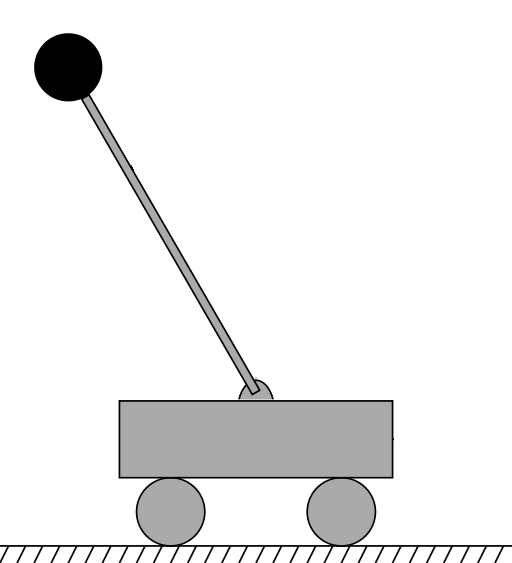
\includegraphics[width=0.5\textwidth]{arrows}
    \caption{\label{arrows} Forces on the cart and the pole, visualized.}
\end{figure}

\begin{equation} \label{state_representation}
    \displaystyle
    \begin{bmatrix}
        \theta \\
        \dot \theta \\
        x _c \\
        \dot x _c
    \end{bmatrix}
    := \begin{bmatrix}
        \theta \\
        \dot \theta \\
        x _c \\
        \dot x _c
    \end{bmatrix}
    + \begin{bmatrix}
        0 & 1 & 0 & 0 \\
        \frac{g}{l} & 0 & 0 & 0 \\
        0 & 0 & 0 & 1 \\
        0 & 0 & 0 & 0
    \end{bmatrix}
    \begin{bmatrix}
        \theta \\
        \dot \theta \\
        x _c \\
        \dot x _c
    \end{bmatrix}
    + \begin{bmatrix}
        0 \\
        - \frac{1}{l} \\
        0 \\
        \frac{1}{M + m}
    \end{bmatrix}
    \begin{bmatrix}
        F
    \end{bmatrix}
\end{equation}

Thus, we have our values for $A$ and $B$:

\begin{equation}
    \displaystyle A = \begin{bmatrix}
        0 & 1 & 0 & 0 \\
        \frac{g}{l} & 0 & 0 & 0 \\
        0 & 0 & 0 & 1 \\
        0 & 0 & 0 & 0
    \end{bmatrix}
\end{equation}

\begin{equation}
    \displaystyle B = \begin{bmatrix}
        0 \\
        - \frac{1}{l} \\
        0 \\
        \frac{1}{M + m}
    \end{bmatrix}
\end{equation}

\section{Control}

\subsection{Objective}

While the model of the environment is complete, we currently have no way to control it. To use the basic state space control law in Equation \ref{control_law}, we need the controller gain matrix $K$ and the reference $\vec{r}$. Our objective is to find values of $K$ and $\vec{r}$ such that the pole will remain in a stable, upright state, and reach it as quickly as possible with minimal error.

\subsection{Reference}

The reference vector $\vec{r}$ is easy to find: in the pole balancing problem, one usually wants to bring the angle, angular speed, position, and positional speed all to zero. This is a stable state, and centers the cart within the bounds of the track. Thus, we simply define $\vec{r}$ as a vector of zeroes:

\begin{equation}
    \displaystyle
    \vec{r} = \begin{bmatrix}
        0 \\
        0 \\
        0 \\
        0
    \end{bmatrix}
\end{equation}

\subsection{Controller Gain Matrix}

\subsubsection{Concept}

Finding the controller gain matrix $K$ is clearly the most difficult part of developing a state space controller. In Equation \ref{control_law}, we can see that it is a matrix mapping the error of the current states off the reference to the input $u$. More intuitively, it can be thought of as a linear regression of the states, used to calculate the best possible input.

\subsubsection{Linear-Quadratic Regulator}

Rather than being trained as in a typical linear regression, an optimal value for $K$ can be found using a control law called Linear-Quadratic Regulator (LQR). Like a linear regression, LQR optimizes a cost function. However, rather than requiring training data extracted from a model of the environment, LQR can optimize $K$ using only the state-space model matrices $A$ and $B$, alongside two cost matrices defined by the developer.

The cost function optimized is as follows:

\begin{equation}
    J = \int _0 ^{\infty} \! (\vec{x} ^T Q \vec{x} + \vec{u} ^T R \vec{u}) \, dt
\end{equation}

This amounts to a summation of the errors in the states and outputs from their references over an infinite period of time.

$Q$ and $R$ are diagonal matrices that define the costs of large errors for each of the states and outputs, respectively. Specifically, the $k$th value in $Q$ defines the contribution to the loss function of the $k$th state.

I used Bryson's rule \cite{veness}, which says that, for a given state with a maximum acceptable value of $z$, the loss coefficient should be $\displaystyle \frac{1}{z ^2}$. After some empirical optimization, I settled on the following values for Q and R:

\begin{equation}
    Q = 40 \begin{bmatrix}
        1 & 0 & 0 & 0 \\
        0 & \frac{1}{9} & 0 & 0 \\
        0 & 0 & \frac{1}{100} & 0 \\
        0 & 0 & 0 & \frac{1}{400}
    \end{bmatrix}
\end{equation}

\begin{equation}
    R = \begin{bmatrix}
        \displaystyle
        \frac{1}{100}
    \end{bmatrix}
\end{equation}

Given values for $Q$ and $R$, the optimal controller gain matrix $K$ was calculated using the Python Control library.

\section{Results}

\subsection{Trial and Error}

The first time I implemented this system, I made two fundamental mistakes:

\begin{itemize}
    \item I thought that Equation \ref{state_derivative} yielded $\vec{x}$ itself rather than $\dot{\vec{x}}$, so I added the identity matrix to $A$.
    \item I made the incorrect assumption, in my environment matrices, that $l$ was equal to 1.
\end{itemize}

Despite these errors, the controller still made all states converge to zero, which says something very significant about the robustness of closed-loop control systems. However, it was slow to approach zero. When I fixed these errors, the stability of the system and the rate of convergence drastically improved.

\subsection{Results (Actually)}

After these issues were fixed, and after some empirical tweaking of the cost matrices $Q$ and $R$, I found that the resulting controller gain matrix $K$ was a very nearly optimal solution to the environment, bringing the pole to the center of the track very rapidly and with very minimal overshoot. Indeed, within 10 seconds all variables have settled to values within a rounding error of zero.

Figures \ref{position}, \ref{angle}, and \ref{force} display this graphically. Raw numbers can be found in Table \ref{motion_statistics}. The beginning conditions were: $x _c = -8$ (quite close to the track boundary, which is at -10) and $\theta = 0$.

\begin{center}
    \begin{tabular}{|l|l|l|l|}
        \hline
        Time (s) & $x _c$ & $\theta$ & $F$ \\
        \hline
        0.00 & -8.00 & 0.00 & -50.60 \\
        \hline
        1.00 & -6.62 & 0.16 & 1.54 \\
        \hline
        2.00 & -3.32 & -0.12 & -1.52 \\
        \hline
        3.00 & -1.14 & -0.13 & -1.40 \\
        \hline
        4.00 & -0.20 & -0.07 & -0.72 \\
        \hline
        6.00 & 0.09 & -0.01 & -0.05 \\
        \hline
        8.00 & 0.02 & 0.00 & 0.02 \\
        \hline
        10.00 & 0.00 & 0.00 & 0.00 \\
        \hline
    \end{tabular}
    \captionof{table}{Raw statistics of changes in variables over time.} \label{motion_statistics}
\end{center}

\begin{figure}[H]
    \centering
    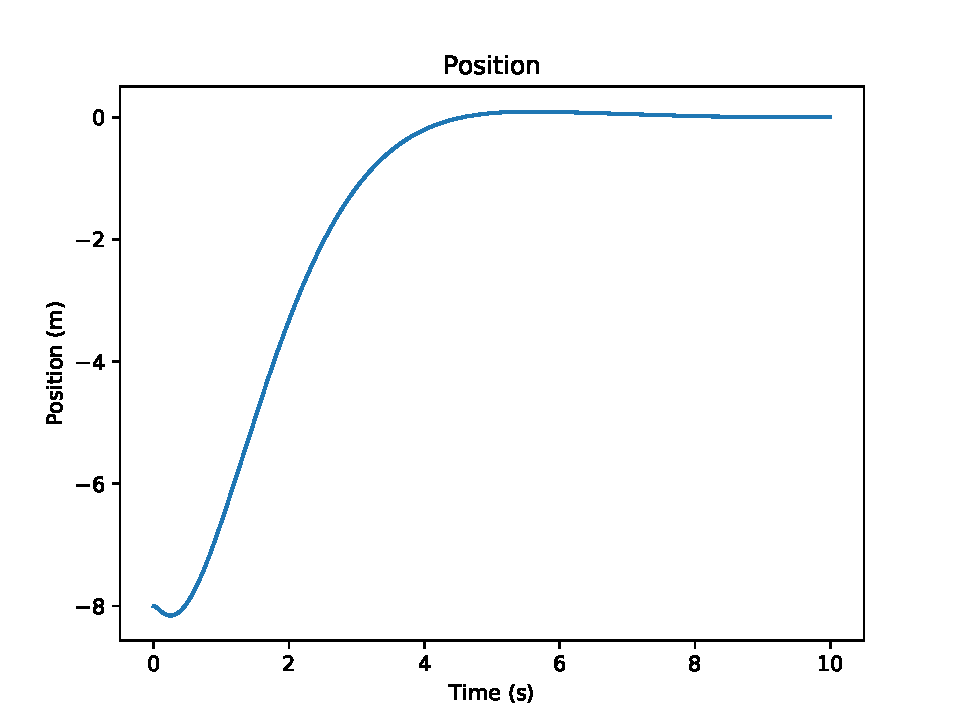
\includegraphics[width=0.8\textwidth]{position}
    \caption{\label{position} A graphical representation of changes in $x _c$ over time.}
\end{figure}

\begin{figure}[H]
    \centering
    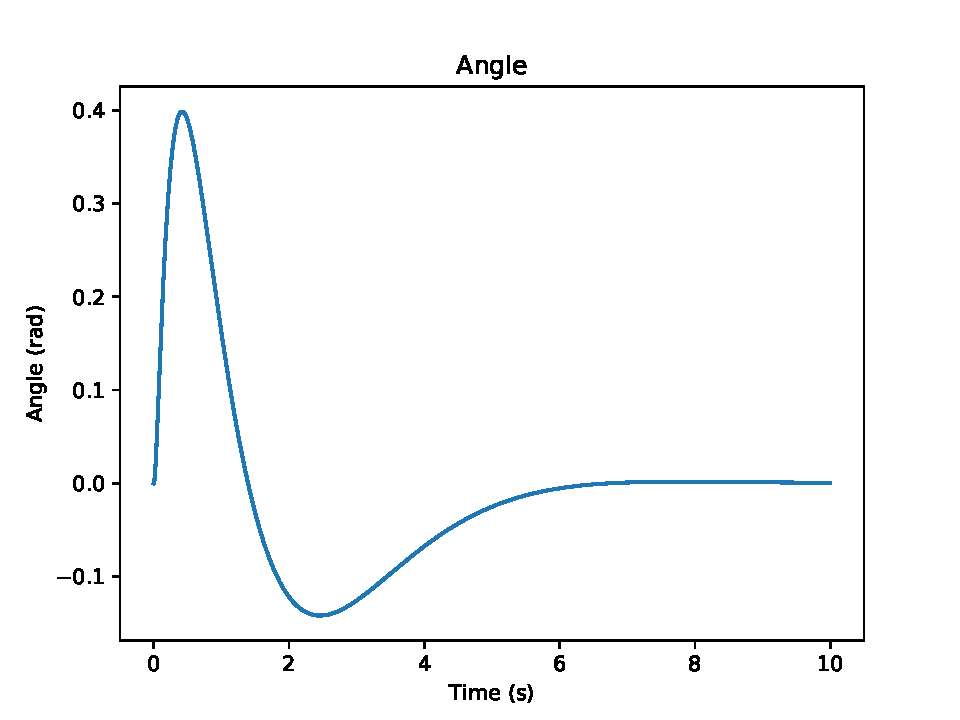
\includegraphics[width=0.8\textwidth]{angle}
    \caption{\label{angle} A graphical representation of changes in $\theta$ over time.}
\end{figure}

\begin{figure}[H]
    \centering
    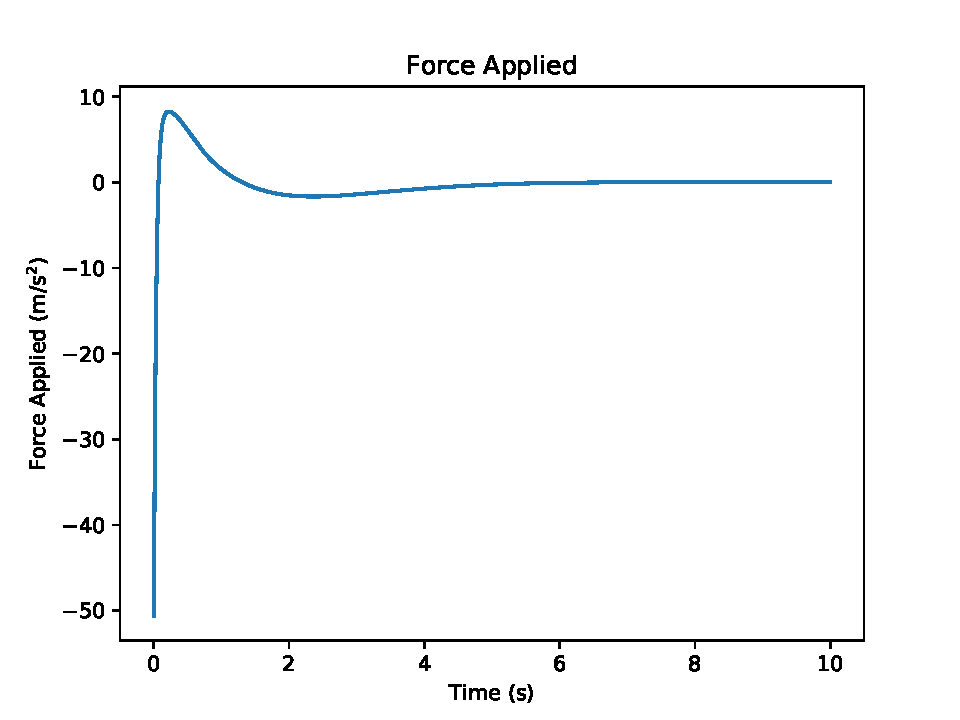
\includegraphics[width=0.8\textwidth]{force}
    \caption{\label{force} A graphical representation of changes in $F$ over time.}
\end{figure}

\section{Conclusions}

These results confirm and demonstrate that linear state space control can indeed make for a robust solution to nonlinear physical environments such as the pole balancing problem. After expressing the environment as a set of linear matrices and applying the LQR optimizer, I have developed a controller that drives all states to the reference efficiently and with very minimal overshoot.

The main implications of these results lie in how they can be expected to generalize to other nonlinear control tasks. As mentioned in Section \ref{problem}, the pole balancing problem has a great deal in common with problems such as bicycle control and humanoid robots, so this result may suggest that state space and LQR have applicability to those challenges.

State space is also used for other diverse subfields of physical control. For instance, the Ramsete controller \cite{ramsete}, which was used by FRC Team 254 for control of four-wheeled non-holonomic robots, is based on state space with modifications for nonlinear path following.

In the future, I hope to investigate other applications for state space and LQR, such as autonomous vehicles. I also hope to learn more about nonlinear control algorithms, and understand where they can, and should, be used instead of linear control.

\printbibliography

\end{document}